\section{GraphBLAS objects}
\label{sec:GrBObjects}

The GraphBLAS C API is built on objects exposed as opaque data types. 
These objects include
\begin{itemize}
\item \emph{Collections}: vectors and matrices.
\item \emph{Algebraic objects}: unary and binary operators, monoids, and semirings.
\item \emph{Control objects}: descriptors and masks (both one- and two-dimensional).
\end{itemize}

Functions that manipulate GraphBLAS objects
are referred to as {\it methods}.  These methods define the 
interface to create or destroy GraphBLAS objects, modify their 
contents, and copy the contents of opaque objects into non-opaque  
objects (i.e. under direct observation and control of the programmer).

\subsection{Collections}
\label{Sec:Collections}

The state of a GraphBLAS application is largely captured by collections of values, 
namely vectors and matrices.  The GraphBLAS collections 
are opaque objects only accessible through the methods in the GraphBLAS C API.
The use of opaque data types gives the implementation the flexibility needed to 
aggressively optimize for different systems.

A GraphBLAS vector $\vector{v} = \langle D, N, \{ (i,v_i) \} \rangle$ is defined by:
\begin{itemize}
\item The domain $D$, i.e. the data type for the vector elements.
\item The size $N>0$.
\item A set of tuples $(i,v_i)$ where $0 \leq
i < N$ and $v_i \in D$. 
\end{itemize}
A particular value of $i$ can only appear 
once in $\vector{v}$. We define $\mathbf{nelem}(\vector{v}) = N$ and
$\mathbf{L}(\vector{v}) = \{ (i,v_i) \}$. The set $\mathbf{L}(\vector{v})$ is
called the \emph{content} of vector $\vector{v}$. 
%%%%
% TGM:  Any concepts we don't use in the paper should not be introduced, 
% hence why these are commented out
%%%%
%We also define the set:
%$$
%\vector{ind(\vector{v})} = \{ i : (i,v_i) \in \mathbf{L}(\vector{v}) \}
%$$
%(called the \emph{structure} of $\vector{v}$), and $\mathbf{D}(\vector{v})
%= D$. 
For a vector $\vector{v}$, $\vector{v}(i)$ is a reference to $v_i$
if $(i,v_i) \in \mathbf{L}(\vector{v})$ and is undefined otherwise. 

A GraphBLAS matrix  $\matrix{A} = \langle D, M, N, \{ (i,j,A_{ij}) \} \rangle$ is
defined by:
\begin{itemize}
\item The domain $D$, i.e. the data type for the matrix elements.
\item The number of rows $M>0$ and columns $N>0$.
\item A set of tuples $\mathbf{L}(\matrix{A}) = (i,j,A_{ij})$ where $0 \leq i < M$, $0 \leq
j < N$, and $A_{ij} \in D$. 
\end{itemize}
A particular pair of values $i,j$ can
only appear once in $\matrix{A}$. 
The set $\mathbf{L}(\matrix{A})$ is called the
\emph{content} of matrix $\matrix{A}$.  
We define $\mathbf{nrows}(\matrix{A}) = M$ and 
$\mathbf{ncols}(\matrix{A}) = N$.
%%%%%
% TGM: if we don't use a notation in this paper, then I don't want to introduce it
%%%%%
%We define $\mathbf{ncols}(\matrix{A})
%= N$,  $\mathbf{nrows}(\matrix{A}) = M$ and $\mathbf{L}(\matrix{A}) =
%\{ (i,j,A_{ij}) \}$.  
%We also define the sets:
%$$
%\vector{indrow(\matrix{A})} = \{ i : \exists (i,j,A_{ij}) \in \matrix{A} \}
%$$
%$$
%\vector{indcol(\matrix{A})} = \{ j : \exists(i,j,A_{ij}) \in \matrix{A} \}
%$$  
%These are the sets of nonempty
%rows and columns of $\matrix{A}$, respectively.)  The \emph{structure}
%of matrix $\matrix{A}$ is the set 
%$$
%\mathbf{ind}(\matrix{A}) = \{ (i,j) :(i,j,A_{ij}) \in \mathbf{L}(\matrix{A}) \}
%$$
%and $\mathbf{D}(\matrix{A}) = D$.
For a matrix $\matrix{A}$, $\matrix{A}(i,j)$ is a reference to $A_{ij}$
if $(i,j,A_{ij}) \in \mathbf{L}(\matrix{A})$ and is undefined otherwise.  
This points to an important and fundamental difference between the GraphBLAS and 
traditional sparse matrix libraries for which elements that are not
explicitly stored are assumed to have the numerical value $0$.   As we will see in
section~\ref{Sec:AlgebraicObjects}, by specifying these
elements as undefined, we avoid the complexity of interpreting implied
values in the sparse array definition differently as the semiring changes.

If $\matrix{A}$ is a matrix and $0 \leq j < N$, then 
$$ \matrix{A}(:,j)= \langle D, M, \{(i,A_{ij}) : (i,j,A_{ij}) \in \mathbf{L}(\matrix{A})\} \rangle
$$
is a vector called the $j$-th \emph{column}
of $\matrix{A}$. Correspondingly, if $\matrix{A}$ is a matrix and
$0 \leq i < M$, then 
$$
\matrix{A}(i,:) = \langle D, N, \{(j,A_{ij}) :(i,j,A_{ij}) \in \mathbf{L}(\matrix{A}) \} \rangle
$$ 
is a vector called
the $i$-th \emph{row} of $\matrix{A}$.

We define the transpose of a matrix in the traditional manner where
row and column indices are swapped.   Consider a matrix 
$
\matrix{A} = \langle D, M, N, \{ (i,j,A_{ij}) \} \rangle,
$;
the \emph{transpose} of $\matrix{A}$ is the matrix 
$$
\matrix{A}^T = \langle D, N, M, \{(j,i,A_{ij}) : (i,j,A_{ij}) \in \mathbf{L}(\matrix{A}) \} \rangle.
$$

\subsection{Algebraic objects}
\label{Sec:AlgebraicObjects}

The GraphBLAS differs from traditional sparse linear algebra APIs in that the
algebra associated with the data can be varied to match the needs
of an application.  This provides a great deal of flexibility 
in the domains for the elements of GraphBLAS
collections and the operators defined between these elements.

We start with  basic binary and unary operators.  
A GraphBLAS \emph{binary operator} is defined as:
$$
F_b = \langle D_1, D_2, D_3, \odot \rangle.
$$
It has three domains, $D_1$, $D_2$, $D_3$, and an operation
$$
\odot: D_1 \times D_2 \rightarrow D_3.
$$
%For a given GraphBLAS operators
%$$
%F_b=\langle D_1, D_2, D_3,\odot \rangle
%$$ we define $\mathbf{D}_1(F_b) = D_1$,
%$\mathbf{D}_2(F_b) = D_2$, $\mathbf{D}_3(F_b) = D_3$, and $\mathbf{\bigodot}(F_b)
%= \odot$.  Note that $\odot$ could be used in place of either $\oplus$ or $\otimes$.
A GraphBLAS \emph{unary operator} is defined as:
$$
F_u = \langle D_1, D_2, f\rangle.
$$
It has two domains, $D_1$, $D_2$, and an operation
$f: D_1 \rightarrow D_2$.  
%For a given GraphBLAS operators
%$$
%F_u=\langle D_1, D_2, f \rangle
%$$ we define $\mathbf{D}_1(F_u) = D_1$,
%$\mathbf{D}_2(F_u) = D_2$, and $\mathbf{f}(F)
%= f$.
%
GraphBLAS makes use of two fundamental algebraic structures: monoids
and semirings.   
A GraphBLAS  \emph{monoid} 
$$
M =\langle D_1,\odot,\mathbf{0} \rangle
$$ 
is defined by a single domain $D_1$, an 
\emph{associative}\footnote{It is expected that implementations 
will utilize IEEE-754 floating point arithmetic, which is not 
strictly associative.} 
operation $\odot: D_1 \times D_1 \rightarrow D_1$,
and an identity element $\mathbf{0} \in D_1$.  
%For a given GraphBLAS monoid
%$$
%M=\langle D_1,\odot,0 \rangle
%$$ 
%we define $\mathbf{D}_1(M) = D_1$, $\mathbf{\bigodot}(M) =
%\odot$ and $\mathbf{0}(M) = 0$.  
Let
$
F = \langle D_1,D_1,D_1,\odot \rangle
$ 
be a GraphBLAS binary operator and let
$\mathbf{0}$ be the identity for $\odot$. Then 
$$
M = \langle F,\mathbf{0} \rangle = \langle
D_1,\odot,\mathbf{0} \rangle
$$ 
is the associated GraphBLAS monoid.

The algebraic structure at the core of the GraphBLAS is the semiring.  
A GraphBLAS \emph{semiring} 
$$
S=\langle D_1,D_2,D_3,\oplus,\otimes,\mathbf{0} \rangle
$$ 
is defined by
three domains $D_1$, $D_2$ and $D_3$, an \emph{associative}
additive operation 
$$
\oplus : D_3 \times D_3 \rightarrow D_3
$$
a multiplicative operation 
$$\otimes : D_1 \times D_2 \rightarrow
D_3
$$
and an element $\mathbf{0} \in D_3$, which is the identity for $\oplus$.
%For a given GraphBLAS semiring 
%$$
%S=\langle D_1,
%D_2, D_3,\oplus,\otimes,0 \rangle
%$$ 
%we define $\mathbf{D}_1(S) = D_1$,
%$\mathbf{D}_2(S) = D_2$, $\mathbf{D}_3(S) = D_3$, $\mathbf{\bigoplus}(S) =
%\oplus$, $\mathbf{\bigotimes}(S) = \otimes$, and $\zero(S) = 0$. 
Let $F = \langle D_1,D_2,D_3,\otimes \rangle$ be a GraphBLAS binary operator,
and let $M = \langle D_3,\oplus,\mathbf{0} \rangle$ be a GraphBLAS monoid;
then 
$$
S= \langle M,F \rangle = \langle D_1,D_2,D_3,\oplus,\otimes,\mathbf{0} \rangle
$$
is a GraphBLAS semiring.
Conversely, for a GraphBLAS semiring 
$S = \langle D_1,D_2,D_3,\oplus,\otimes,\mathbf{0} \rangle$,
there is always an associated monoid 
$M = \langle D_3,\oplus,\mathbf{0} \rangle$ and
an associated binary operator $F = \langle D_1,D_2,D_3,\otimes \rangle$.

A UML diagram of the conceptual hierarchy of algebraic objects in GraphBLAS
algebra 
%(binary operators, monoids and semirings) 
is shown in 
Figure~\ref{Fig:AlgebraHierarchy}.  Note that GraphBLAS semiring differs from 
the fundamental algebraic semiring in that the GraphBLAS semiring (i) 
allows input from different domains and can produce an output in a third
domain, and (ii) does not require the definition of the
multiplicative annihilator.


\begin{figure}[htb]
    %\hrule
    \begin{center}
        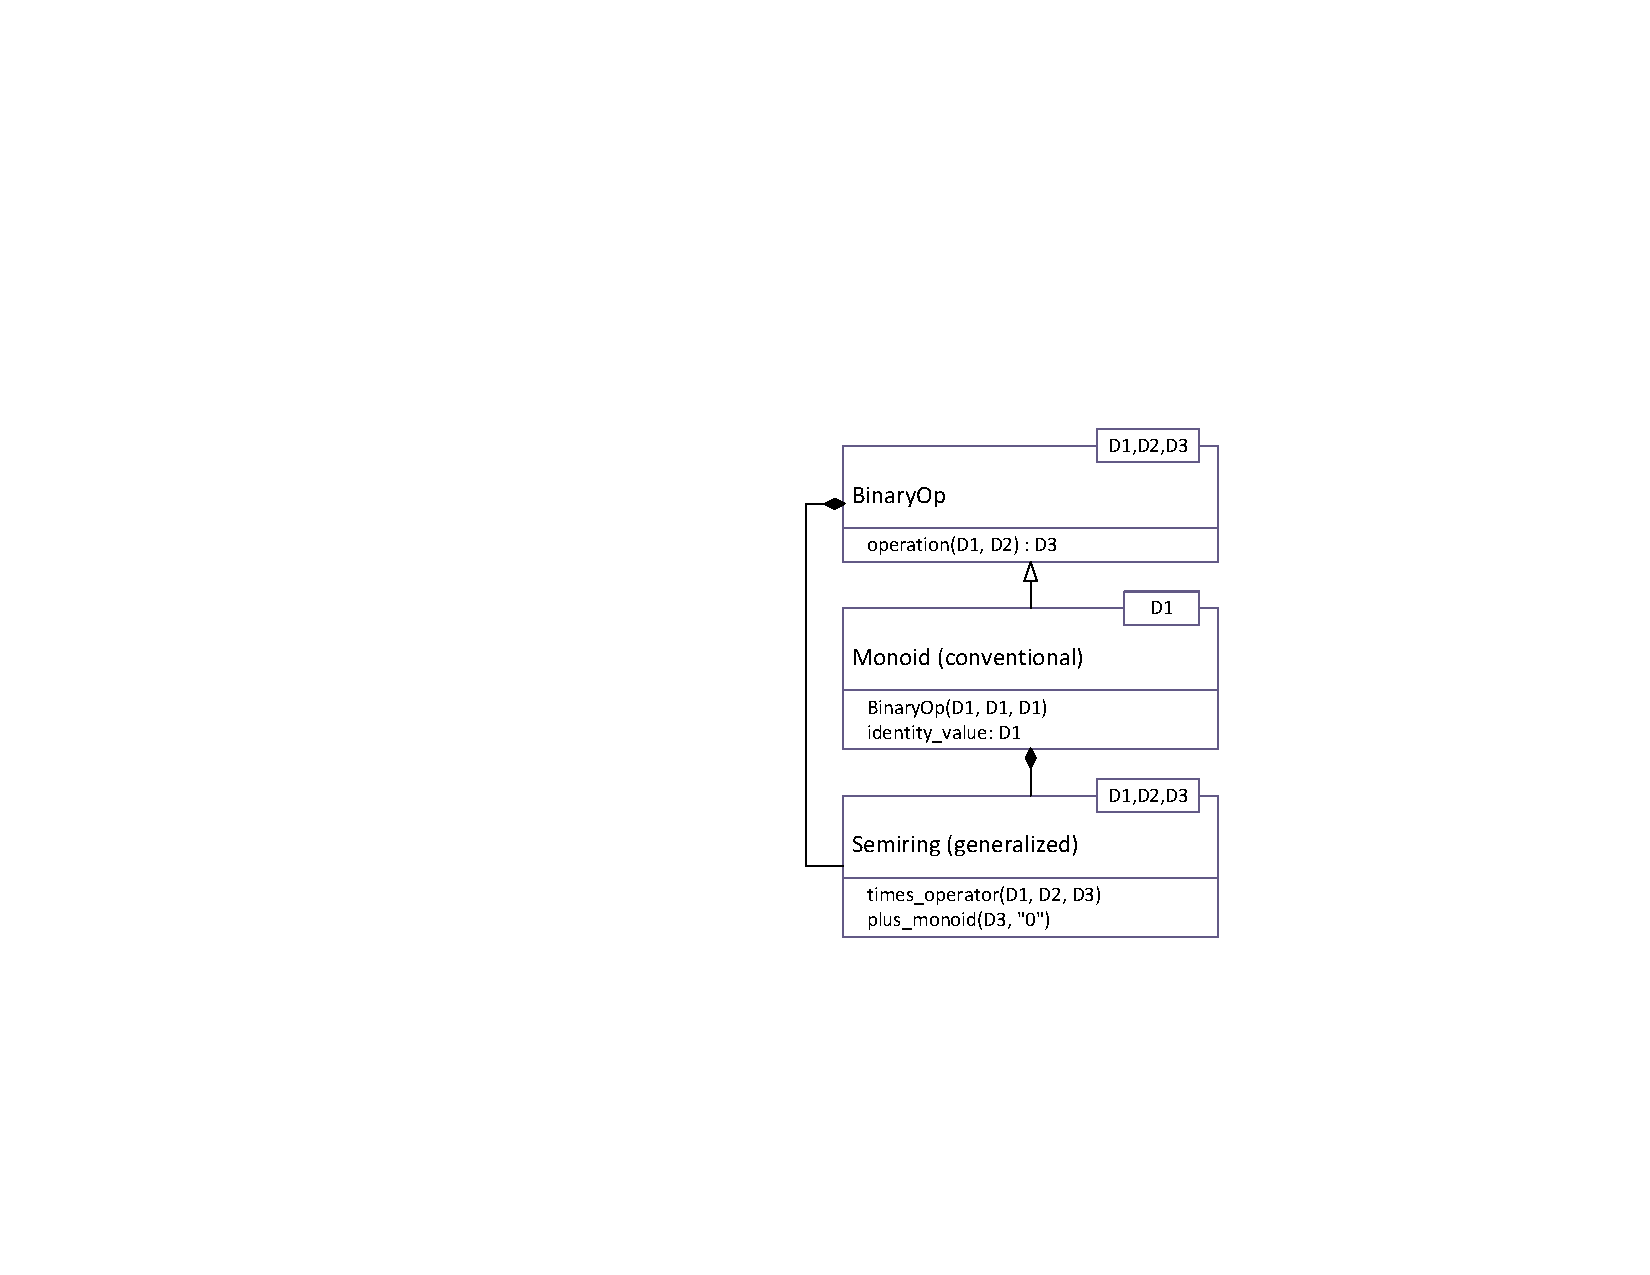
\includegraphics[width=0.58\linewidth]{Algebra_Hierarchy_v2.pdf}
    \end{center}
    \vspace{-4pt}
    \caption{Hierarchy of algebraic object classes in GraphBLAS. GraphBLAS semirings consist of a conventional monoid with one domain for the addition function, and a binary operator with three domains for the multiplication function.}
    \label{Fig:AlgebraHierarchy}
    \vspace{-4pt}
    %\hrule
\end{figure}


\subsection{Control objects}
\label{Sec:ControlObjects}

The GraphBLAS C API defines two opaque objects that 
modify the semantics of GraphBLAS methods; \emph{masks} and 
\emph{descriptors}.  

A mask can be either a one- or a two-dimensional construct.  One- and
two-dimensional masks, described more formally below, are similar to
vectors and matrices, except that they have structure
(indices) but no values. Masks are used to control which values from 
a operation are written to the output object.

A one-dimensional mask $\vector{m} = \langle N, \{ i \} \rangle$ is
defined by its number of elements $N>0$ and a set $\mathbf{L}(\vector{m})$
of indices $\{ i \}$ where $0 \leq i < N$.  A particular value of $i$ can
appear at most once in $\vector{m}$. We define $\mathbf{nelem}(\vector{m})
= N$.  
We define the \emph{structure} of a one dimensional mask as the set
$\mathbf{L}(\vector{m})$.
%% JEM: For masks, L(m) and ind(m) are identical. Let us see if we can avoid defining ind(m).
%% $$
%% \vector{ind(\vector{m})} = \{ i : i \in
%% \mathbf{L}(\vector{m}) \}
%% $$
A two-dimensional mask
$
\matrix{M} = \langle M, N, \{ (i,j) \}
\rangle
$
is defined by its number of rows $M>0$, its number of
columns $N>0$, and a set $\mathbf{L}(\matrix{M})$ of tuples $(i,j)$
where $0 \leq i < M$, $0 \leq j < N$.   A particular pair of values
$i,j$ can appear at most once in $\matrix{M}$.  
%We define
%$\mathbf{ncols}(\matrix{M}) = N$, and $\mathbf{nrows}(\matrix{M}) = M$.
The \emph{structure} of a two-dimensional mask $\matrix{M}$ is the set
$\mathbf{L}(\matrix{M})$.
We also define $\mathbf{nrows}(\matrix{M}) = M$ and
$\mathbf{ncols}(\matrix{M}) = N$.
%% $$
%% \mathbf{ind}(\matrix{M}) = \{ (i,j) : (i,j) \in \mathbf{L}(\matrix{M}) \}
%% $$

Operations may be directed to use the \emph{structural complement} of a mask.
For a one-dimensional mask, $\vector{m}$, this is denoted as
$\neg\vector{m}$. For a two-dimensional mask, $\matrix{M}$, this is denoted as
$\neg\matrix{M}$.  The structure of the complement of an one-dimensional
mask $\vector{m}$ is defined as:
$$
\mathbf{L}(\neg\vector{m}) = \{i : 0
\leq i < N, i \notin \mathbf{L}(\vector{m}) \}
$$
It is the set of all
possible indices that do not appear in $\vector{m}$.  The structure
of the complement of a two-dimensional mask $\matrix{M}$ is defined as:
$$
\mathbf{L}(\neg\matrix{M}) = \{(i,j) : 0 \leq i < M, 0 \leq j < N,
(i,j) \notin \mathbf{L}(\matrix{M}) \}
$$
It is the set of all possible indices that do not appear in $\matrix{M}$.

The second control object is the \emph{descriptor}.  Descriptors
modify the semantics of GraphBLAS methods by controlling additional optional behaviors. 
In particular, descriptors specify how other input arguments 
-- vectors, matrices and masks -- should be processed (modified) 
before the main operation of a method is performed.  It is
also used to specify whether the output argument should be cleared before assignment.

The descriptor is a lightweight object.  It pairs a set of flags
representing the possible modifiers with each mask, vector, or matrix argument of a
GraphBLAS method.  For example, a descriptor may specify that a particular 
input matrix needs to be transposed or that the structural compliment of a mask should be used.

For the descriptors, the arguments of a method
are identified through the field names. The output parameter (typically
the first parameter in a GraphBLAS method) is indicated by the field name, 
{\sf GrB\_OUTP}, the mask by {\sf GrB\_MASK} field name, and the input 
vectors and matrices by {\sf GrB\_INP0}
and {\sf GrB\_INP1} (in the order they appear in the signature of the method).
A code example, showing the creation of a descriptor can be found on 
lines~\ref{line:bfs_desc}-\ref{line:bfs_desc_end} of Figure~\ref{Fig:BClisting}.

\section{GraphBLAS Execution Model}
\label{sec:GrBExec}

Algorithms are expressed as one or more \emph{sequences} of GraphBLAS 
method calls.  The methods within a sequence occur in the order they are encountered 
in the program (the \emph{Program Order}).  A new sequence begins with the 
first method that creates or modifies a GraphBLAS object and
terminates with a call to the {\sf GrB\_wait()} method.  New sequences can begin
following termination of a prior sequence, hence sequences
within a single thread are contiguous and do not overlap.  A multithreaded
program may have a distinct sequence per thread, but those sequences
must not share objects unless the shared objects are read-only.

Each method in a sequence and the inputs to the method uniquely and unambiguously
defines the output GraphBLAS objects.  
A GraphBLAS program executes in one of 
two modes: \emph{blocking} and \emph{nonblocking}.  
\begin{itemize}
\item \emph{blocking}: Each method in a sequence completes the GraphBLAS operation 
before proceeding to the next statement in program order.  Output GraphBLAS
objects are in memory and available to other C statements after each method returns.

\item \emph{nonblocking}: Methods \emph{may} return once input arguments 
have been verified.   Methods that only manipulate opaque objects \emph{may} defer their 
execution.  Methods that input non-scalar, non-opaque objects or output non-opaque objects may not defer their execution. 
When a method is deferred, values associated with the method's
output GraphBLAS objects  are undetermined until: (1) the sequence is terminated, or (2) a GraphBLAS method 
that copies values from a GraphBLAS object into a non-opaque object returns.   At that point, the GraphBLAS object 
is said to be \emph{complete}, i.e. values associated with that object are in memory and available
to subsequent C functions.  
\end{itemize}

In a  mathematically well-defined sequence with input objects that are numerically well-conditioned, the results
from blocking and nonblocking modes should be identical other than effects due to round-off errors 
associated with floating point arithmetic.   

Blocking mode forces an implementation to carry out precisely the GraphBLAS operations
defined by the methods and to store output objects to memory between method calls.  
It is valuable for debugging or when an external tool needs to 
evaluate the state of memory during a sequence.

Nonblocking mode gives an implementation flexibility to choose
an execution strategy that might reduce the time required to execute the methods 
in a sequence.  Methods may be placed into
a queue and deferred.  They can be chained together and fused (\eg,
replacing a chained pair of matrix products with a matrix triple product).
Lazy evaluation, greedy evaluation, and asynchronous execution are all
valid as long as the final result agrees with the mathematical 
definition provided by the sequence of GraphBLAS method calls.

A conforming implementation of the GraphBLAS C API running in 
nonblocking mode may choose to execute ``as if'' in blocking mode.   
Furthermore, a sequence in nonblocking mode where
every GraphBLAS operation is followed by a call to  {\sf GrB\_wait()} 
is equivalent to the same sequence in blocking mode without the calls to {\sf GrB\_wait()}.

The mode is defined in the GraphBLAS C API when the context of the library invocation 
is defined.  This occurs once before any GraphBLAS methods are called with a call to the
{\sf GrB\_init()} function.   After all GraphBLAS methods are complete, the context is terminated
with a call to {\sf GrB\_finalize()}.  The context can only be 
set once in the execution of a program; i.e. after {\sf GrB\_finalize()} is called, a subsequent call to
{\sf GrB\_init()} is not allowed.

\section{Error Model}
\label{sec:GrBError}

GraphBLAS methods return a value of type {\sf GrB\_Info} to provide information 
about the execution of a method available 
at the time the method returns.� The specification of each method lists the allowed return values. 
Errors fall into two classes: \emph{API errors} and \emph{execution Errors}.  An API error
means a GraphBLAS method was called with parameters that violate the
rules for that method. Execution errors indicate that something
went wrong during the execution of a legal GraphBLAS method invocation.
Their occurrence may depend on specifics of the executing environment.
This does not mean that environment errors are the fault of the GraphBLAS
implementation.  For example, a memory leak is a program error, but it
may manifest itself in different points of program execution (or not at
all) depending on the platform, problem size, or what else is running
at that time.

When a GraphBLAS method is called, the arguments are evaluated
for any API errors.  If any API errors 
are found, the method returns without making any changes to the method's
arguments and with a return value corresponding to the appropriate 
API error.   If  API errors are not found, the method can proceed to carry out the
computation associated with the method.

In blocking mode the computation for each method proceeds after testing for any
API errors.  When the method is finished, it returns the
value {\sf GrB\_SUCCESS} if the computation completed without errors. 
If an execution error was found, the method returns
a value to indicate the appropriate execution error.

In nonblocking mode, we distinguish between methods that may defer execution (i.e.
methods that only read and write opaque objects) and methods that may not defer
execution (i.e. methods that read input arrays or methods that force completion of 
a GraphBLAS object).  If the methods allow deferred execution, API errors are tested when the method
is called.  If no API errors are found, the method returns with the value 
of {GrB\_SUCCESS}.  Since execution in nonblocking mode may be deferred, the only 
information available when a method returns pertains to the API test; i.e. the return value does not provide 
any information  about the status of the computation.

When the sequence is terminated by a call to {\sf GrB\_wait()} a value of
{\sf GrB\_SUCCESS} is returned if no execution errors were encountered in 
the execution of the sequence.  Other return values from {\sf GrB\_wait()}indicate an error occurred
during execution of the sequence.  Additional information may be available by 
a call to the method {\sf GrB\_error()} which returns a pointer to a null terminated 
string containing any additional error information that might be available.  

Methods in nonblocking mode that do not allow deferred execution 
carry out the computation associated with the method after tests for 
API errors.  When these methods force completion of a GraphBLAS 
object (such as methods to extract values from an opaque object into a non-opaque object)
the return value is {GrB\_SUCCESS} if no execution errors were generated by any 
of the methods involved in defining the mathematical value of the completed GraphBLAS object.
If execution errors were encountered, a return value indicates that an error condition was encountered
and, as with the call to {\sf GrB\_wait()}, additional information may be provided by a call to
{\sf GrB\_error()}.



